\documentclass[12pt,a4paper,titlepage,brazil]{article}
\usepackage[a4paper]{geometry}
\geometry{top=2.0cm, bottom=2.0cm, left=2cm, right=2cm}
\usepackage{tabularx} 
\usepackage{multicol}
\usepackage{multirow}
\usepackage{longtable}
\usepackage{threeparttablex}
\usepackage{array}
\usepackage{graphicx}
\usepackage{caption}
\usepackage[english]{babel} 
\usepackage[T1]{fontenc}
\usepackage[utf8]{inputenc}
\usepackage[a4paper]{geometry}
\geometry{top=2.0cm, bottom=2.0cm, left=2.0cm, right=2.0cm}
\usepackage{setspace}
\usepackage{hyperref}
\usepackage[ttscale=.85]{libertine}
\usepackage{libertinust1math}
\usepackage[table]{xcolor}

\begin{document}

\begin{center}
 \huge{\textbf{First steps on GitHub}}\\
 \large{Natalí S. M. de Santi (\href{https://github.com/natalidesanti}{\texttt{@natalidesanti}})}
\end{center}

All steps below are for passionate by terminal on {\bf Linux} operational system.

%%%%%%%%%%%%%%%%%%%%%%%%%%%%%%%%%%%%

\section{Step 1 - What is GitHub?}

\begin{minipage}{0.7\textwidth}
{\bf GitHub} is a code hosting platform for version control and collaboration using {\bf git}. It lets you and others work alone or together on projects from anywhere.

{\bf Git} is a distributed version-control system for tracking changes in source code during it development. It is designed for coordinating work among programmers, but it can be used to track changes in any set of files. Its goals include speed, data integrity and support for distributed non-linear workflows.\\
\end{minipage}
\begin{minipage}{0.3\textwidth}
 \vspace{-0.5cm}
 \centering    
 
\includegraphics[scale=0.22]{github-logo.png}\\
\href{https://www.flaticon.com/authors/dave-gandy}{GitHub logo.}
\end{minipage}

%%%%%%%%%%%%%%%%%%%%%%%%%%%%%%%%%%%%

\section{Step 2 - Creating a GitHub account}

To start your experience on {\bf GitHub} you need to make an account on:
\url{https://github.com}. You will just need to inform your \texttt{e-mail} account, choose an \texttt{username} and create a \texttt{password}. Now, instead of using your password to do your git things, you will need to use your \texttt{token}. The instructions to do this are available in the \href{https://docs.github.com/en/github/authenticating-to-github/creating-a-personal-access-token}{page}.

%%%%%%%%%%%%%%%%%%%%%%%%%%%%%%%%%%%%

\section{Step 3 - Installing git in your computer}

You need to install {\bf git} in your computer. If you are using {\bf Ubuntu} you just need to run OS and package updates:\\

\texttt{\$ sudo apt-get update}\\

And install {\bf git} giving the following command:\\

\texttt{\$ sudo apt-get install git-core}\\

You may be asked to confirm the download and installation. {\bf Git} should be installed and ready to use. If you can confirm it you can just run the {\bf git} version command:\\

\texttt{\$ git -\hspace{0.01cm}-version}\\

Mine is:\\

\texttt{\$ git version 2.25.1}.

%%%%%%%%%%%%%%%%%%%%%%%%%%%%%%%%%%%%

\section{Step 4 - Creating a repository}

After creating an account you need to start a first (or new) {\bf repository} on {{\bf GitHub}. A repository is usually used to organize a {\bf project}. Repositories can contain anything your project needs: folders, files, images, videos, data sets, etc.

You can create your repository in the {\bf GitHub} \href{https://github.com}{site}, giving to it the following features:
\begin{itemize}
 \item Name: \texttt{project\_name}.
 \item Description: ``\texttt{This project has the objective to...}''.
 \item Privacy: \texttt{public} (anyone can see this repository, but you can choose who can commit) or \texttt{private} (you choose to see and commit to this repository);
 \item README;
 \item LICENSE;
\end{itemize}
The last two options are really useful if the project is not only yours, or even if you want to share it with anyone else. I prefer always create this things after, because then you will end up in a page that gives you the {\bf link} (and some instructions) of your project, that you will use in your computer, to indicates where it will be online! But, as the link is the same as the project one, fell free to create these files whatever time that you want.

Just to know, the \texttt{README}, i.e, a file with information about your project, which is written in \texttt{markdown}. The \texttt{license} gives the rights about what other people can do or not with your work. Some directions about what license chose can be found in the \href{https://opensource.guide/legal/#which-open-source-license-is-appropriate-for-my-project}{page} and the instructions to add one in your repo is \href{https://docs.github.com/en/github/creating-cloning-and-archiving-repositories/licensing-a-repository}{here}.

Then, you need to start a first (or new) repository giving, inside the directory, in your computer, chosen by you, the command:\\

\texttt{\$ git init}\\

Now you need to say who you are for your {\bf git}. Write in the terminal:\\

\texttt{\$ git config -\hspace{0.01cm}-global user.email <you@example.com>}

\texttt{\$ git config -\hspace{0.01cm}-global user.name <your\_name>}\\

You need to pay attention that \texttt{-\hspace{0.01cm}-global} means that you are using {\bf git} on your computer. If you omit this option you are logging in only on the local folder.\\

If you want to see the user and the configuration of your {\bf git}, access the file \texttt{\~\/.gitconfig} and the information will be like:\\

\texttt{[user]}\\

\hspace{0.5cm}\texttt{email = you@example.com}\\

\hspace{0.5cm}\texttt{name = your\_name}\\

%%%%%%%%%%%%%%%%%%%%%%%%%%%%%%%%%%%%

\section{Step 5 - Including files in your repository}

You need to add the files that you wish to keep your changes on {\bf git}, giving the command:\\

\texttt{\$ git add <file\_name>}\\

Remember that, in other times (beyond the first one), when you are adding the changes you need to write \texttt{stage}, instead \texttt{add}, in the command above, like:\\

\texttt{\$ git stage <file\_name>}

%%%%%%%%%%%%%%%%%%%%%%%%%%%%%%%%%%%%

\section{Step 6 - Committing}

On {\bf GitHub}, saved changes are called {\bf commits}. Each commit has an associated {\bf commit message}, which is a description explaining why a particular change was made. Commit messages captures the history of your changes, so you and other contributors can understand what you’ve done and why.\\

After adding/staging you need to commit it:\\

\texttt{\$ git commit -m ``<message>''}\\

You can do as many commits as you want, giving the command above and writing a message to warn you about your changes, in same documents, or about new documents added in your repository.

%%%%%%%%%%%%%%%%%%%%%%%%%%%%%%%%%%%%

\section{Step 7 - Uploading your files and changes to GitHub}

It's time to upload your {\bf git} on {\bf GitHub}. Now you need to log in on {\bf GitHub} site, access your project and upload your {\bf git} giving the commands sequence:\\

\texttt{\$ git remote add origin https://github.com/user/project\_name.git}

\texttt{\$ git push -u origin master}\\

{\bf GitHub} will ask for your \texttt{username} and  \texttt{password}\footnote{Remember to use your \texttt{token} instead your \texttt{password}!}:\\

\texttt{Username for 'https://github.com': username}

\texttt{Password for 'https://username@github.com': password}\\

And then, you can see which files and commits were upload by you:\\

\texttt{Counting objects: N, done.}
  
\texttt{Delta compression using up to M threads.}

\texttt{Compressing objects: 100\% (N/N), done.}

\texttt{Writing objects: 100\% (O/O), 1.46 KiB | 374.00 KiB/s, done.}

\texttt{Total N (delta 0), reused 0 (delta 0)}

\texttt{To https://github.com/username/project\_name.git}

\texttt{* [new branch]      master -> master}

\texttt{Branch 'master' set up to track remote branch 'master' from 'origin'.}\\

The {\bf git}'s magic works in this way: you create or add some files, modify them, commit your changes and upload the files on {\bf GitHub}. But there is a lot more!

%%%%%%%%%%%%%%%%%%%%%%%%%%%%%%%%%%%%

\section{Step 8 - Not uploading some files and changes to GitHub}

Sometimes you want to hide some files, i.e., files that are not important/necessary for the whole project. Then, you just need to create a {\bf .gitignore} file, specifying the files that you want to ignore. Here you have two options, create this file before everything, if you already know the files that you do not want or create this file after some time. If you are in the former situation, you just need to write in the terminal:\\

\texttt{\$ touch .gitignore}\\

Open it in your favorite text editor and specify the files. For instance:\\

\texttt{*.log}\\

\texttt{*.aux}\\

\texttt{*.out}\\

If you are in the ``else'' case, before writing anything in your {\bf .gitignore} file, please, delete the files from your git using:\\

\texttt{\$ git rm file\_name.extension}\\

Then, proceed specifying the files to ignore.

%%%%%%%%%%%%%%%%%%%%%%%%%%%%%%%%%%%%

\section{Step 9 - Creating a branch}

Now you need to know that all that you have done above was made in the \texttt{master} branch. Ops, what I'm talking about?

{\bf Branching} is the way to work on different versions of a repository at one time. By default your repository has one \texttt{branch} named {\bf master} which is considered to be the {\em definitive branch}. We use branches to experiment and make edits before committing them to \texttt{master}. In other words, in {\bf git} you can have a tree history of your code. As a tree you have not only one, but a lot of branches. In the branches you can do changes in your files, save them and use it in your \texttt{master} branch as you want.

When you create a branch off the \texttt{master} branch, you’re making a copy of master as it was at that point in time. If someone else made changes to the master branch while you were working on your branch, you could {\bf pull} in those updates. But it is a story that I will tell to you in the next steps.\\

First, we are going to create a branch:\\

\texttt{\$ git branch <name\_of\_branch>}\\

Second, you need to get to that branch:\\

\texttt{\$ git checkout <name\_of\_branch>}\\

Then, you can stage, commit and push files to that branch, using the same commands used right above. Just notice that, when you do your \texttt{push} you just need to change \texttt{master} by your current brunch \texttt{name\_of\_branch}:\\

\texttt{\$ git push -u origin <name\_of\_branch>}\\

You can add as many branches as you want, like direct and different branches from \texttt{main} or even branches starting in other branches. Just remember that, for each branch that you create, the files in that branch will be the same ones in the previous branch as you start your modifications and commits on it.

You can see all branches of your project writing in the terminal:\\

\texttt{\$ git branch}\\

and the present branch that you are working in will be presented with a \* at the left side as:

\texttt{\* master}\\

\texttt{branch 1}\\

\texttt{branch 2}\\

\texttt{branch 3}\\

If you want to delete some branch you just need to write:\\

\texttt{\$ git branch -d <name\_of\_branch>.}

%%%%%%%%%%%%%%%%%%%%%%%%%%%%%%%%%%%%

\section{Step 10 - Merging}

As I have described in the previous step, after all changes and commits in your branch, you can put the modifications in the \texttt{main} one. You just need to \texttt{merge} the main with the branch that you are using. Thus, in the main branch you can give the line command:

\texttt{\$ git merge name\_of\_branch}

Finally, you have the \texttt{main} branch completely changed by your other branch changes!

\begin{figure}[h!]
 \centering 
 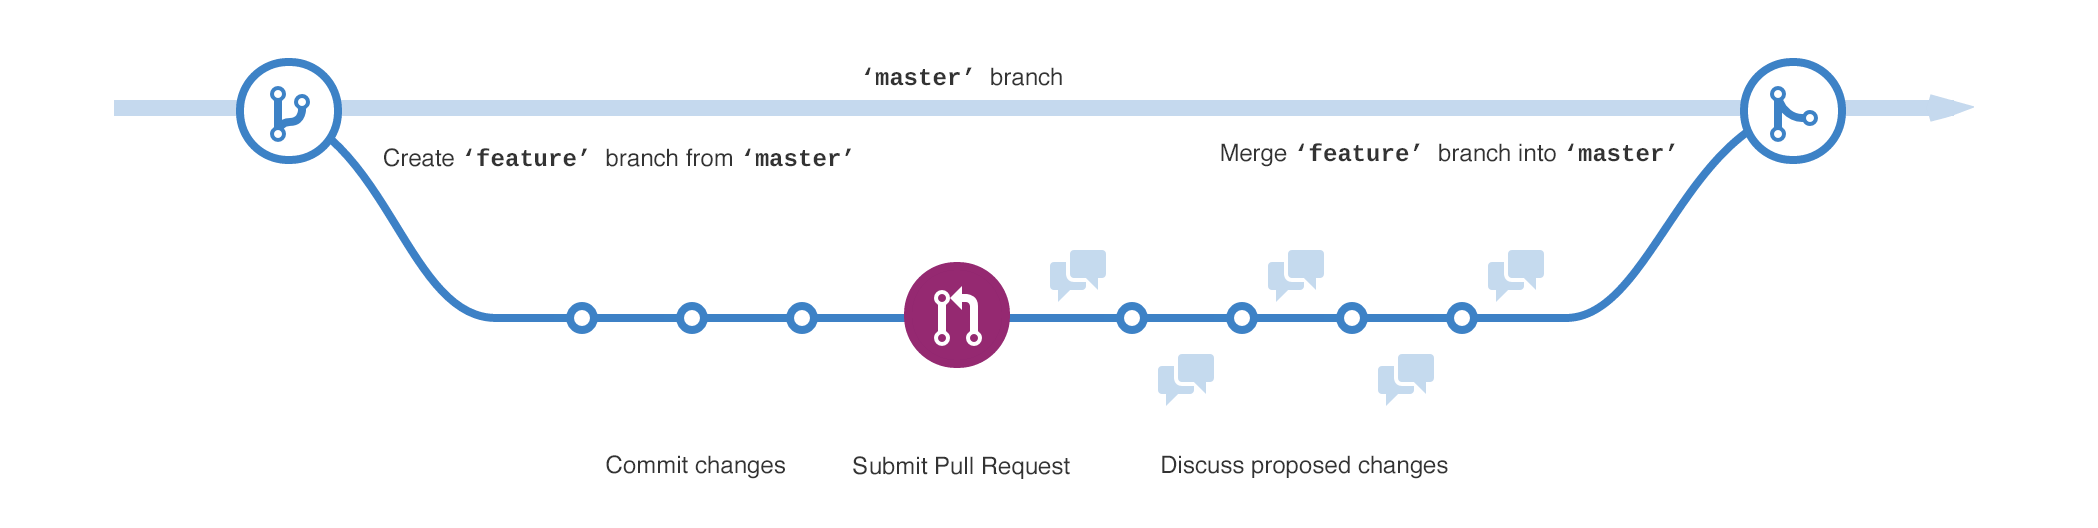
\includegraphics[scale=0.24]{branching.png}
 \caption{Master branch side by side another branch in which there are many commits, pull requests and discussion before merging into the main one. This image is from \texttt{Hello Word project on GitHub's \href{https://guides.github.com/activities/hello-world/branching.png}{site}}.}
\end{figure}

Pay attention that, the command \texttt{merge}, merges the branch that you are in with the other branch you chose, i. e., you can add the changes of the chosen branch in the branch that you are in, and not just for the \texttt{main} branch and the other one desired branch.\\

If you need to verify in which branch you are, what files were be uploaded or not and how they are in your {\bf GitHub}'s page, you can just write in the terminal:

\texttt{\$ git status}.

%%%%%%%%%%%%%%%%%%%%%%%%%%%%%%%%%%%%

\section{Step 11 - Pull Requests}

{\bf Pull Requests} are the heart of collaboration on {\bf GitHub}. When you open a pull request, you’re proposing your changes and requesting that someone, really anyone, review and pull in your contribution and merge them into their branch. Pull requests show diffs, or differences, of the content from both branches. The changes, additions, and subtractions are shown in {\color{green}green} and {\color{red}red} in your {\bf GitHub}'s page.

As soon as you make a commit, you can open a pull request and start a discussion, even before the code is finished.

By using {\bf GitHub}’s \texttt{@mention} system in your pull request message, you can ask for feedback from specific people or teams.

You can even open pull requests in your own repository and merge them yourself. It’s a great way to learn the {\bf GitHub} flow before working on larger projects.

Again, there is a lot of other things to do on {\bf git} and {\bf GitHub}.

%%%%%%%%%%%%%%%%%%%%%%%%%%%%%%%%%%%%

\section{Step 12 - Changing}

If you are using {\bf git} you certainly will do changes in your project. Then, you can use the following commands:

\begin{itemize}
 \item To show the differences in file that are not realized yet:\\
   \texttt{\$ git diff};
 \item To show the differences in staged files and its last versions:\\
   \texttt{\$ git diff -\hspace{0.01cm}-staged};
 \item Unselect the file, preserving its content:\\
   \texttt{\$ git reset <file\_name>};
 \item To remove the file:\\
   \texttt{\$ git rm <file\_name>};
 \item To remove the file, preserving it locally:\\
   \texttt{\$ git rm -\hspace{0.01cm}-cached <file\_name>};
 \item To change the file name and to select it to a new commit:\\
   \texttt{\$ git mv <original\_file\_name> <new\_file\_name>};
 \item Undo all commits after the specified commit, keeping the local changes:\\
   \texttt{\$ git reset <commit>};   
 \item Discards every history and changes for the specified commit:\\
   \texttt{\$ git reset -\hspace{0.01cm}-hard <commit>}.   
\end{itemize}  

%%%%%%%%%%%%%%%%%%%%%%%%%%%%%%%%%%%%

\section{Step 13 - Saving fragments}

You can still save and restoring incomplete changes using:

\begin{itemize}
 \item Keeps, temporally, all modified files:\\
   \texttt{\$ git stash};
 \item Restores all recent files that have been stashed:\\
   \texttt{\$ git stash pop};
 \item List all changes in stash:\\
   \texttt{\$ git stash list};
 \item Discards every recent settle of changes in stash:\\
   \texttt{\$ git stash drop}.
\end{itemize}  

%%%%%%%%%%%%%%%%%%%%%%%%%%%%%%%%%%%%

\section{Step 14 - Reviewing history}

You can make a review of the evolution of all files in some {\bf git} project using:

\begin{itemize}
 \item List the versions history in the local branch:\\
   \texttt{\$ git log};
 \item List the history versions for specific file, including name alterations:\\
   \texttt{\$ git log -\hspace{0.01cm}-follow <file\_name>};
 \item Show the differences between the content among two branches:\\
   \texttt{\$ git diff <first\_branch> \dots <second\_branch>};
 \item Show the changes in the metadata and content for the specif commit:\\
   \texttt{\$ git show <commit>}.
\end{itemize}  


%%%%%%%%%%%%%%%%%%%%%%%%%%%%%%%%%%%%

\section{Step 15 - Forking/Cloning a repository}

If you are surfing into {\bf GitHub}'s site and find a great project that you like you can {\bf fork/clone} it for you. Then, you will have this repo into your computer to run, to modify and to do whatever you want without affecting the original project. To fork/clone some repo you need to follow two steps:

\subsection{Forking:}

Navigate until the {\bf GitHub} project that you liked and, in the top-right corner of the page, click {\bf Fork}!

\subsection{Cloning:}

To be ``connected'' with that repo and receive the last actualization's of it, when the owner do some modifications, i.e., to keep your fork synced, you just need to write in the terminal:\\

\texttt{\$ git clone <link>}.\\

This command do the download of the project with its complete historic version. As a simple example, you can clone this tutorial writing:\\

\texttt{\$ git clone <https://github.com/natalidesanti/first\_steps\_on\_github>}.\\

Remember to clone some repo in some location that you want into your computer.\\

If you have interest to make a pull request in this repo you can give:\\

\texttt{\$ git pull}\\

to see the last alterations into this repo before proceed to make your pull request!\\

If you want to clone a specific branch the command line is:\\

\texttt{\$ git clone -\hspace{0.05cm}-branch <branchname> <remote-repo-url>}\\

%%%%%%%%%%%%%%%%%%%%%%%%%%%%%%%%%%%%

\section{Backing in time}

One of the options that have helped me a lot is using the \texttt{HEAD} option. I use this when I make a tremendous mistake and \texttt{git} helps me to keep everything on the track. So, if I make a commit that I do not want to miss but I need the before ones, I come back in time using:\\

\texttt{\$ git stash}\\

And create a branch with the previous commit using:\\

\texttt{\$ git checkout HEAD$\sim$N}\\

where $N$ indicates the number of the commits that I want to back in time. Then, I decide what to do and come back with the desired alteration in the main branch!

%%%%%%%%%%%%%%%%%%%%%%%%%%%%%%%%%%%%

\section{Basic git commands}

I would like to finish this manuscript listing some basic {\bf git commands}:

\begin{table}[h!]
 \begin{center}
  \begin{tabular}{c|c|c}
   \cline{1-3}
   \textbf{Git task} & \textbf{Notes} & \textbf{Git commands} \\
   \cline{1-3}
   Adding & ``*'' means & \texttt{git add <file\_name>}\\
   files & all files & \texttt{git add *}\\
   \cline{1-3} 
   & Create a & \\
   & new branch & \\
   & and switch & \texttt{git checkout -b name\_of\_branch}\\
   & to it & \\
   & or commit & \\
   \cline{2-3}
   & Switch from & \\
   & one branch & \texttt{git checkout name\_of\_branch}\\
   Branches & to another & \\    
   \cline{2-3}
   & List all the & \\
   & branches in & \\
   & your repo & \texttt{git branch} \\    
   & and tell you & \\
   & what branch & \\
   & you are in & \\
   \cline{2-3} 
   & Delete the & \\
   & specific & \texttt{git branch -d name\_of\_branch}\\
   & branch & \\    
   \cline{1-3}
   Create a & & \\
   new local & & \texttt{git init}\\
   repository & & \\
   \cline{1-3} 
   Commit & & \texttt{git commit -m ``<message>''}\\
   \cline{1-3} 
   & To merge a & \\
   & different & \\
   Merge & branch into & \texttt{git merge name\_of\_branch}\\
   & your active & \\
   & branch & \\
   \cline{1-3} 
   & Send changes & \\
   & to the master & \texttt{git push origin master}\\
   Push & branch & \\
   \cline{2-3} 
   & Push the & \\
   & branch to & \texttt{git push origin name\_of\_branch}\\
   & your repo & \\
   \cline{1-3} 
   & List the files & \\
   & you've changed & \\
   Status & and those you & \texttt{git status}\\
   & still need to add & \\
   & or commit & \\
   \cline{1-3}
  \end{tabular}
 \end{center}
\end{table}

\begin{table}[h!]
 \begin{center}
  \begin{tabular}{c|c|c}
   \cline{1-3} 
   & Configure the & \\
   & author name & \\
   Tell git & and email & \texttt{git config -\hspace{0.01cm}-global user.email <you@example.com>}\\
   who you are & address to be & \texttt{git config -\hspace{0.01cm}-global user.name <your\_name>}\\ 
   & used with & \\
   & your commits & \\
   \cline{1-3}
   Undo & Undo the most & \texttt{git reset HEAD$\sim$1}\\
   & recent commit & \\
   \cline{1-3} 
  \end{tabular}
 \end{center}
\end{table}


%%%%%%%%%%%%%%%%%%%%%%%%%%%%%%%%%%%%

\section{Acknowledgments and references}

To write the \textbf{First steps on GitHub} I really appreciate the Nícolas Morazotti (\href{https://github.com/Morazotti}{\texttt{@Morazotti}} help, Patricia Novais (\href{https://github.com/pnovais}{\texttt{@pnovais}}) tutorial, the \href{https://guides.github.com/activities/hello-world/}{\texttt{Hello World}} project and the Wikipedia pages for \href{https://en.wikipedia.org/wiki/GitHub}{GitHub} and \href{https://en.wikipedia.org/wiki/Git}{git}.

\end{document}

%%% Local Variables:
%%% mode: latex
%%% TeX-master: t
%%% End:
